\documentclass{jsarticle}
\usepackage{amsmath, smssymb, amsfonts}
\usepackage{newtxtext, newtxmath}
\usepackage{latexsym}
\usepackage{mathrsfs}
\usepackage{mathtools}
\usepackage{textcomp}
\usepackage{mathcomp}
\usepackage[dvipdfmx]{graphicx, xcolor}
\usepackage{float}
\usepackage{wrapfig}	% must be after float package.
\usepackage{subcaption}
\usepackage{booktabs}
\usepackage{url}
\usepackage{listings, jvlisting, color}

\definecolor{OliveGreen}{rgb}{0.0,0.6,0.0}
\definecolor{Orenge}{rgb}{0.89,0.55,0}
\definecolor{SkyBlue}{rgb}{0.28, 0.28, 0.95}
\lstset{
  language={C++}, % 言語の指定
  basicstyle={\ttfamily},
  identifierstyle={\small},
  commentstyle={\smallitshape},
  keywordstyle={\small\bfseries},
  ndkeywordstyle={\small},
  stringstyle={\small\ttfamily},
  frame={tb},
  breaklines=true,
  columns=[l]{fullflexible},
  numbers=left,
  xrightmargin=0zw,
  xleftmargin=3zw,
  numberstyle={\scriptsize},
  stepnumber=1,
  numbersep=1zw,
  lineskip=-0.5ex,
  keywordstyle={\color{SkyBlue}},     %キーワード(int, ifなど)の書体指定
  commentstyle={\color{OliveGreen}},  %注釈の書体
  stringstyle=\color{Orenge}          %文字列
}


\begin{document}

\title{ゼミ レポート 09}
\author{山田朔也}
\maketitle

\section{本レポートについて}
本レポートは6月28日に行われたゼミにて出題された課題に対するレポートとなっている。
課題内容は、静磁界計算をフーリエ変換を用いて行う事となる。

\section{原理}
\subsection{離散高速フーリエ変換を用いたConvolution演算の高速計算}
\begin{equation}
	\mathrm{A}(i)=\sum_{j=1}^{n} \mathrm{C}(j-i)\cdot \mathrm{B}(j),\;\;\;\;\;\;\;i=1,\cdots,n
	\label{01}
\end{equation}
式\ref{01}の演算において、A,Bはそれぞれ長さ$n$のベクトル、Cは長さ$2n-1$のベクトル、$n$は二の累乗の数とする。
このような演算をConvolution演算と呼び、計算時間は$n$の二乗に比例する。

B及びCが周期$n$の周期関数であるとき、上記の演算は以下の手順で計算することができる。
\begin{enumerate}
	\item B及びCのフーリエ成分Br(実数部),Bi(虚数部),Cr(実数部),Ci(虚数部)を求める。
	\item 求めたフーリエ成分の各成分を直接掛け合わせ、結果をそれぞれAr,Aiとする。
		\begin{align}
			\mathrm{Ar}(i) &= \mathrm{Br}(i)\cdot\mathrm{Cr}(i)-\mathrm{Bi}(i)\cdot\mathrm{Ci}(i),								\notag \\
			\mathrm{Ai}(i) &= \mathrm{Br}(i)\cdot\mathrm{Ci}(i)+\mathrm{Bi}(i)\cdot\mathrm{Cr}(i),\;\;\;\;\;\;\;i=1,\cdots,n	\notag
		\end{align}
	\item Ar,Aiを逆フーリエ変換する。このとき得られた実数部が求めるAとなる。
\end{enumerate}
このときの計算時間は、$\mathrm{O}(n \log (n))$となる。

\subsection{非周期構造でのConvolution演算}
第2章1節では、計算対象が周期構造を持つ場合に適応することができる手法であるが、
以下に述べるゼロパディング手法を用いることで、周期構造を持たない場合も適応できる。

長さ$n$のベクトルBおよびCを例に取る。
まずB,Cを長さ$2n$に拡張し、$\mathrm{B',C'}$とする。
拡張は式\ref{02},\ref{03}のように行う。
\begin{align}
	\mathrm{B':\;B(1),B(2),\cdots,B(n),0,0,\cdots,0}				\label{02} \\
	\mathrm{C':\;0,C(-n+1),C(-n+2),\cdots,C(0),C(1),\cdots,C(n-1)}	\label{03}
\end{align}

ベクトルB',C'の2つを第2章1節の計算手順に従って計算を行い、逆フーリエ変換して得られたベクトルをA'とする。
このとき、$\mathrm{A'(n+1),\cdots,A'(2n)}$の成分が求める演算の解となる。


\section{問題1}
\subsection{問題内容}
問題内容は、3章で行った1次元計算での静磁界計算を、離散高速フーリエ変換を用いて行うものに書き直す。
そして、作成したプログラムを用いて静磁界を求め、従来法で求めたものとほぼ一致するか確認し、計算時間と計算点nとの関係を求める。

\subsection{材料定数}
材料定数は、結果の欄で特筆しない限り以下のものを使用する。
\begin{itemize}
	\item 飽和磁化$M = 800\;\mathrm{emu/cm^3}$
	\item 交換スティフネス定数$A = 1\times 10^{-6}\;\mathrm{erg/cm}$
	\item 異方性定数$K_u = 0\;\mathrm{erg/cm^3}$
	\item 損失定数$\alpha = 1$
	\item 磁気回転比$\lvert\gamma\rvert = 1.76\times 10^7\;\mathrm{rad/(s\cdot Oe)}$
	\item 時間刻み$\mathrm{dt} = 0.1\times 10^{-12}\;\mathrm{s}$
	\item 格子間隔$\mathrm{dx} = 80\;$\AA
	\item 膜厚:Bloch磁壁$\mathrm{dz} = 1000\;$\AA
	\item 膜厚:$\mathrm{N\Acute{e}el}$磁壁$\mathrm{dz} = 100\;$\AA
	\item 計算点数$\mathrm{n} = 30$
	\item 計算の境界では、左端が(0,-1,0)、右端が(0,1,0)を用いる
	\item 初期値(Bloch磁壁):$my$は計算領域内で-1から+1まで直線的に変化、$mz=\sqrt{1-my^2}\,,\,mx=0$
\end{itemize}

\subsection{結果}
まず、離散高速フーリエ変換を用いて求めた静磁界の値と、通常の計算手法を用いて求めた静磁界の値の誤差率を計算した。
ただし、真値は通常の計算手法の方とした。

このときの結果は、-3.156473e-16$\%$となった。
この値は非常に小さく、ほぼ一致したと考えられる。

次に静磁界計算の計算時間と計算点数nの関係を、図\ref{fig01}に示した。
なお、この計算を行うにあたって、計算点数nの値を変えつつ実行している。
\begin{figure}
	\centering
	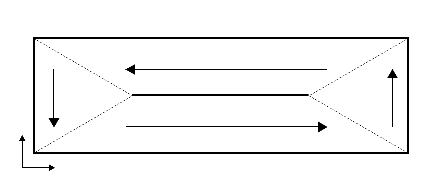
\includegraphics[width=14cm]{pic01.eps}
	\caption{計算時間と計算点nの関係}
	\label{fig01}
\end{figure}

図\ref{fig01}から離散高速フーリエ変換を用いた計算方法を用いることで、
計算数nが肥大化しても、計算時間は通常方法を用いたものより抑えられることがわかる。
また、計算点数nが小さい場合は、通常方法を用いたもののほうが計算時間が短くて済むこともわかった。

\section{問題2}
\subsection{問題内容}
問題内容は5章で作成したプログラムを、静磁界計算を離散高速フーリエ変換を用いて行うものに書き直し、
計算制度、計算時間を調べる事だ。

\subsection{材料定数}
材料定数等は、各小問の欄で特筆しない限り以下のものを使用する。
\begin{itemize}
	\item 計算点がx-y面に広がる2次元計算
	\item 直方体をセルを用いて離散化を行う
	\item 磁気モーメントを求める点は、各計算セルの中心に配置し、磁気モーメントは全て同じ方向を向くと仮定する。
	\item 飽和磁化$M = 800\;\mathrm{emu/cm^3}$
	\item 交換スティフネス定数$A = 1\times 10^{-6}\;\mathrm{erg/cm}$
	\item 異方性定数$K_u = 0\;\mathrm{erg/cm^3}$
	\item 損失定数$\alpha = 1$
	\item 磁気回転比$\lvert\gamma\rvert = 1.76\times 10^7\;\mathrm{rad/(s\cdot Oe)}$
	\item 時間刻み$\mathrm{dt} = 0.1\times 10^{-12}\;\mathrm{s}$
	\item 格子間隔$\mathrm{dx} = 80\;$\AA
	\item 格子間隔$\mathrm{dy} = 80\;$\AA
	\item 格子間隔$\mathrm{dz} = 450\;$\AA
	\item x方向の計算点数$\mathrm{nx} = 48$
	\item y方向の計算点数$\mathrm{ny} = 16$
	\item z方向の計算点数$\mathrm{nz} = 1$
	\item 境界領域では、ノイマン条件を用いる。
	\item 初期値は計算領域の中心を中心として反時計回りの方向を向いている円形状を初期値とし、磁壁の中心部では磁化を多少+z方向に持ち上げておく。
\end{itemize}

\subsection{結果}
まず、離散高速フーリエ変換を用いて求めた静磁界の値と、通常の計算手法を用いて求めた静磁界の値の誤差率を計算した。
ただし、真値は通常の計算手法の方とした。

このときの結果は、1.211736e-10$\%$となった。
この値は非常に小さく、ほぼ一致したと考えられる。

次に静磁界計算の計算時間と計算点数nの関係を、図\ref{fig02}に示した。
なお、この計算を行うにあたって、計算点数nyの値を変えつつ実行している。
それに加え、nyを$1.5\times ny,\,2.0\times ny$と増やした際に、
nzも$1.5\times nz,\,2.0\times nz$と増やすこととした。
\begin{figure}
	\centering
	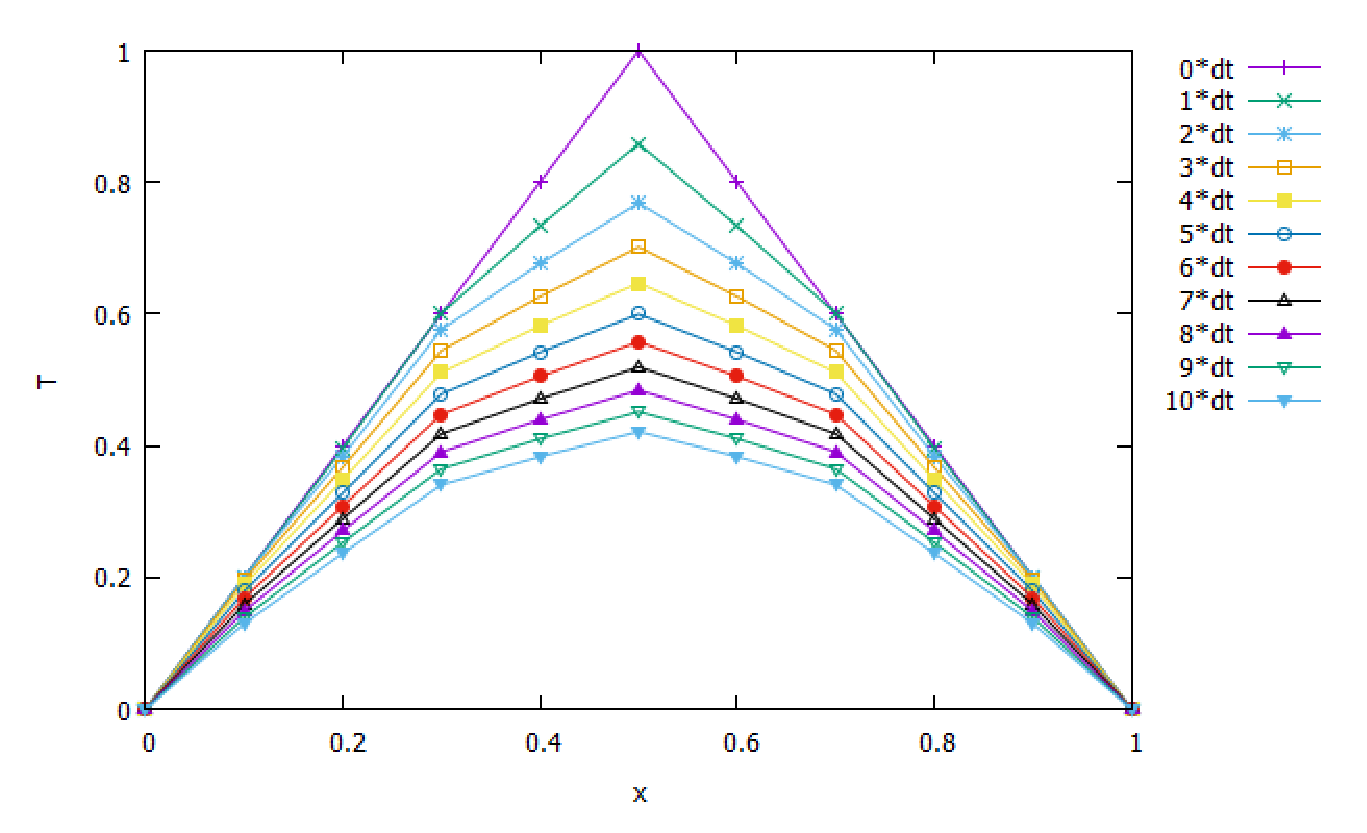
\includegraphics[width=14cm]{pic02.eps}
	\caption{計算時間と計算点nの関係}
	\label{fig02}
\end{figure}

図\ref{fig02}から図\ref{fig01}と同様に、離散高速フーリエ変換を用いた計算方法を用いることで、
計算数nが肥大化しても、計算時間は通常方法を用いたものより抑えられることがわかる。
また、図\ref{fig01}とは異なり、二次元方向に計算をしているため、各軸方向への計算点数が少なくても、
計算時間が長くなりやすい。
よって、計算点数が少ないときでも、離散高速フーリエ変換を用いた計算方法の方が計算時間が短くなる。

\section{問題3}
\subsection{問題内容}
問題内容は、離散高速フーリエ変換を用いて枕木磁壁の磁化構造を求め、直接法の結果と比較する。

\subsection{材料定数}
材料定数は第4章2節に準拠する。

\subsection{結果}
枕木磁壁の計算をした結果を、それぞれ図\ref{fig03_1},\ref{fig03_2}として示す。
\begin{figure}[H]
	\centering
	\begin{subfigure}{0.49\columnwidth}
		\centering
		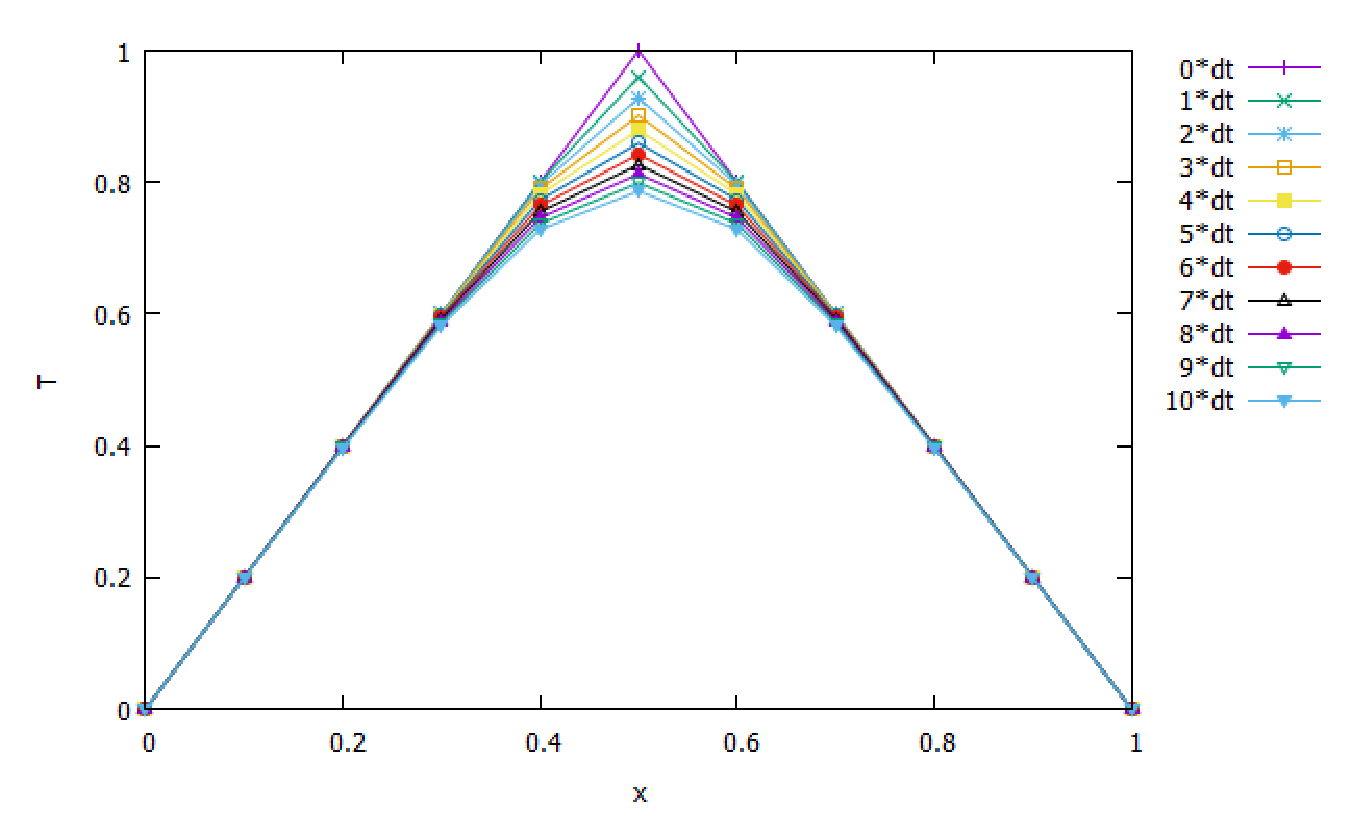
\includegraphics[width=\columnwidth]{pic03.eps}
		\caption{離散高速フーリエ変換を用いて計算した結果}
		\label{fig03_1}
	\end{subfigure}
	\begin{subfigure}{0.49\columnwidth}
		\centering
		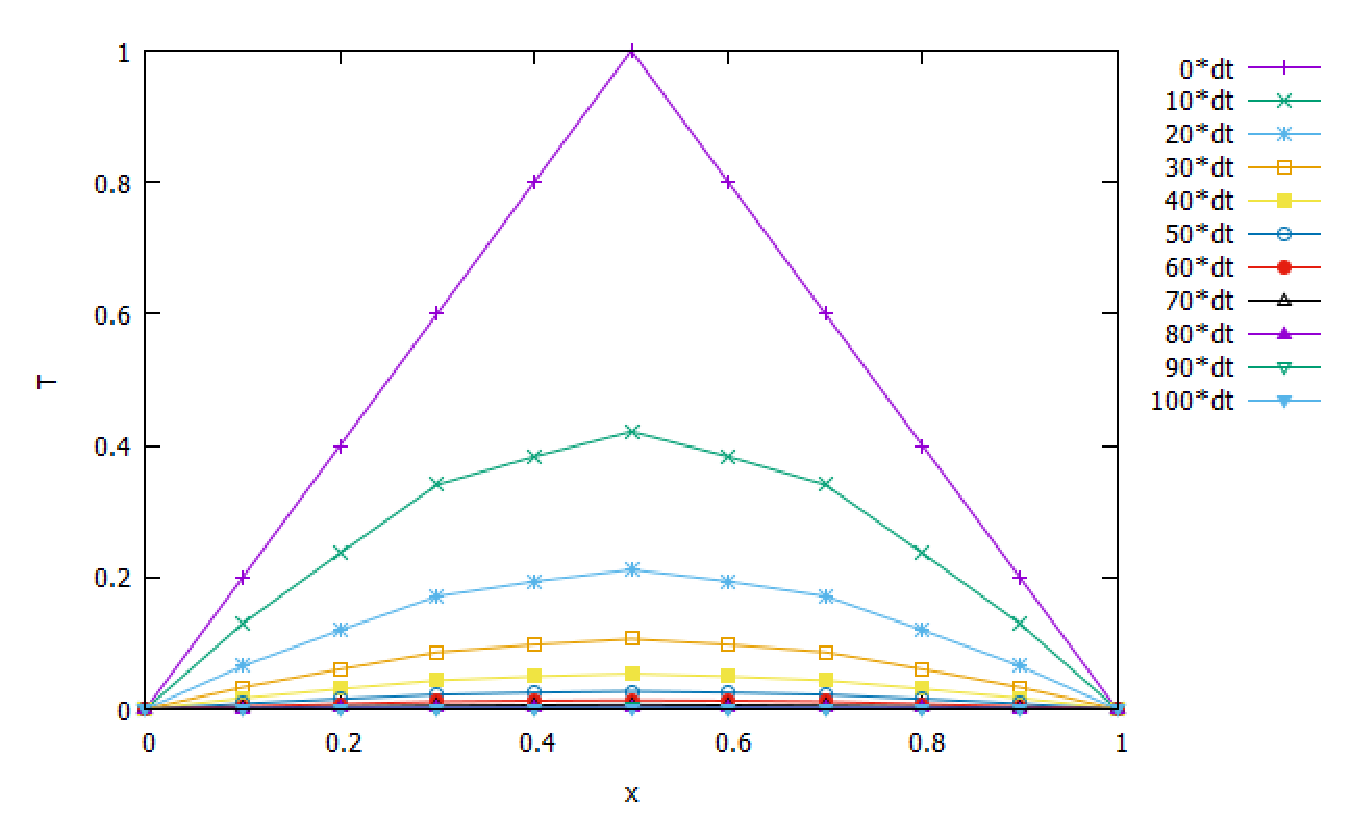
\includegraphics[width=\columnwidth]{pic04.eps}
		\caption{直接法を用いて計算した結果}
		\label{fig03_2}
	\end{subfigure}
	\caption{静磁界係数の計算結果}
	\label{fig03}
\end{figure}

次に、この結果の誤差率を計算したところ、7.577389e-08$\%$となった。

図\ref{fig03}や誤差率からほぼ一致していることが分かる。

\section{参考文献}

\begin{itemize}
  \item 配布されたテキスト
\end{itemize}

\end{document}